\documentclass[tikz, border=0mm]{standalone}
\usepackage{ytableau}
\usetikzlibrary{calc}

\newcommand{\tikzsetnextfilename}[1]{}

\ytableausetup{boxsize=0.99em}

\begin{document}
\tikzsetnextfilename{catabolism}
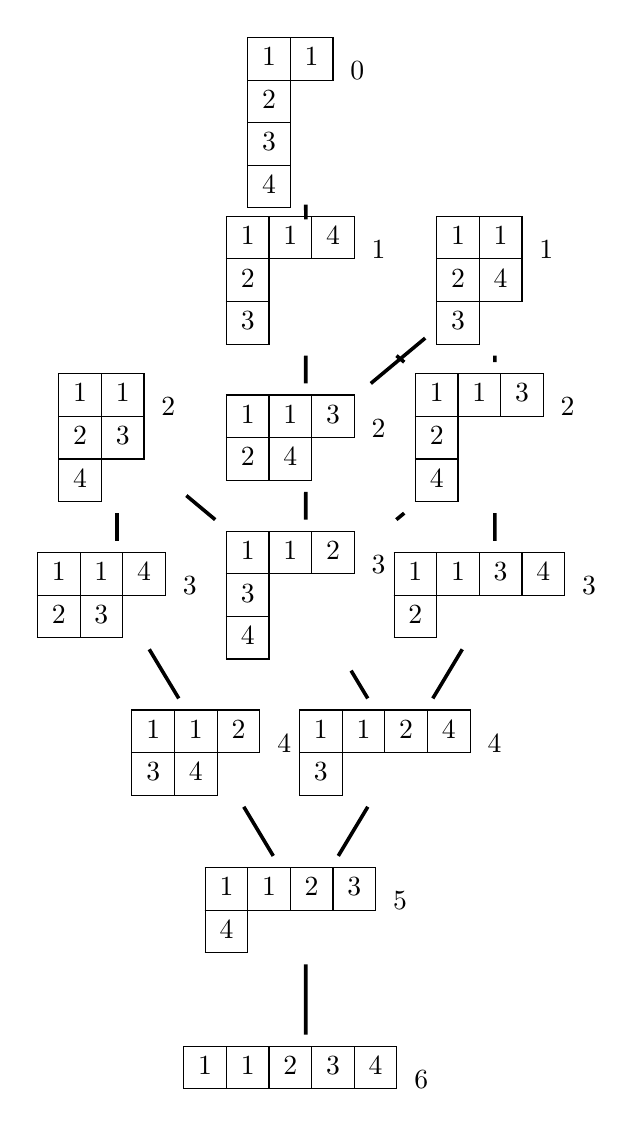
\begin{tikzpicture}[xscale=1.2, yscale=1.0,line width=1.3pt]

\node (R7N1) at (2, 12) {\ytableaushort{11,2,3,4}\; 0};

\node (R6N1) at (2, 10) {\ytableaushort{114,2,3}\; 1};
\node (R6N2) at (4, 10) {\ytableaushort{11,24,3}\; 1};


\node (R5N1) at (0, 8) {\ytableaushort{11,23,4}\; 2};
\node (R5N2) at (2, 8) {\ytableaushort{113,24}\;  2};
\node (R5N3) at (4, 8) {\ytableaushort{113,2,4}\; 2};


\node (R4N1) at (0, 6) {\ytableaushort{114,23}\; 3};
\node (R4N2) at (2, 6) {\ytableaushort{112,3,4}\; 3};
\node (R4N3) at (4, 6) {\ytableaushort{1134,2}\; 3};


\node (R3N1) at (1, 4) {\ytableaushort{112,34}\; 4};
\node (R3N2) at (3, 4) {\ytableaushort{1124,3}\; 4};

\node (R2N1) at (2, 2) {\ytableaushort{1123,4}\; 5};

\node (R1N1) at (2, 0) {\ytableaushort{11234}\; 6};


\draw (R7N1) -- (R6N1);
\draw (R6N2) -- (R5N2);
\draw (R6N2) -- (R5N3);
\draw (R6N1) -- (R5N2);
\draw (R6N1) -- (R5N3);

\draw (R5N1) -- (R4N1);
\draw (R5N1) -- (R4N2);
\draw (R5N2) -- (R4N2);
\draw (R5N3) -- (R4N2);
\draw (R5N3) -- (R4N3);

\draw (R4N3) -- (R3N2);
\draw (R4N2) -- (R3N2);
\draw (R4N1) -- (R3N1);

\draw (R3N2) -- (R2N1);
\draw (R3N1) -- (R2N1);

\draw (R2N1) -- (R1N1);


\end{tikzpicture}




\end{document}
